% 9 variables in here:
% h_1 = 10.0, h_2 = 10.0, h_3 = 10.0, ux_1 = 0.0, ux_2 = 0.0, ux_3 = 2.0, uy_1 = 0.0, uy_2 = 0.0, uy_3 = 0.0
\begin{figure}[ht]
\centering
  \subfigure[1st basis function, $x$-momentum -- 1st basis function, $y$-momentum -- 2nd basis function, $y$-momentum -- 3rd basis function, $y$-momentum] {
    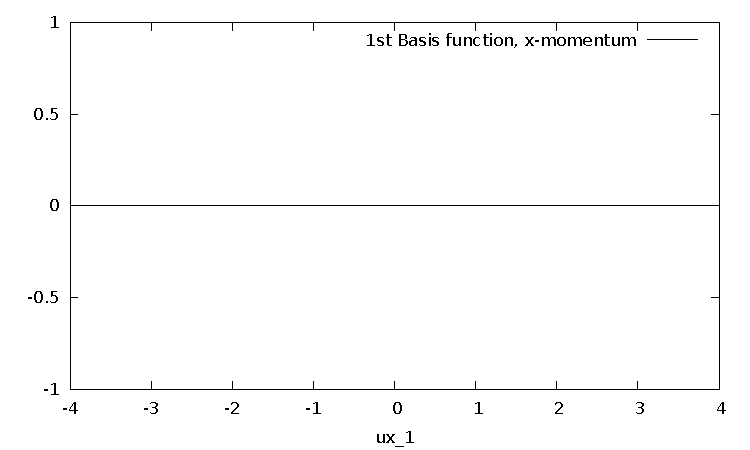
\includegraphics[scale=\zoomfactor]{{{ord1_ux1_differing_ux2_ux3/10.0_10.0_10.0_y_0.0_2.0_0.0_0.0_0.0f00}}}
  }
  % \subfigure[] {
  %   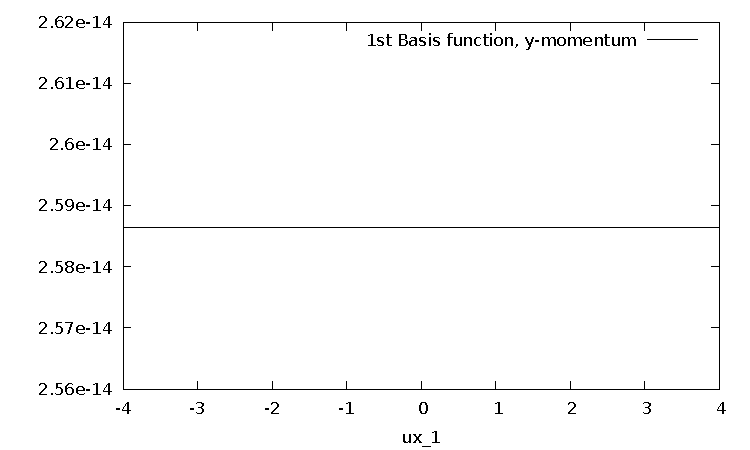
\includegraphics[scale=\zoomfactor]{{{ord1_ux1_differing_ux2_ux3/10.0_10.0_10.0_y_0.0_2.0_0.0_0.0_0.0f01}}}
  % }
  \subfigure[2nd basis function, $x$-momentum -- 3rd basis function, $x$-momentum] {
    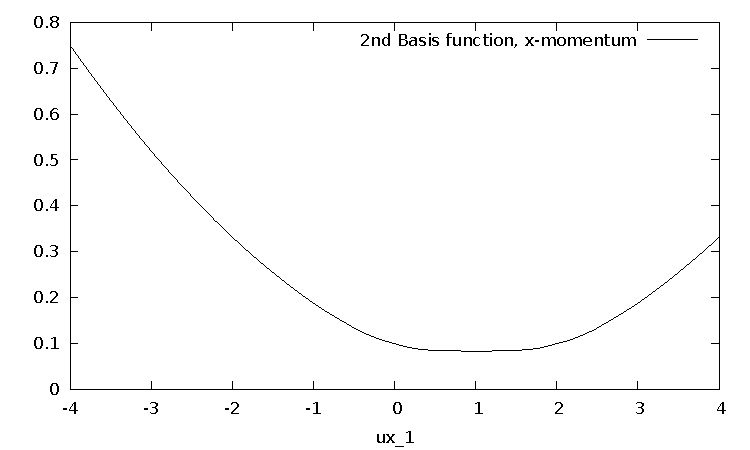
\includegraphics[scale=\zoomfactor]{{{ord1_ux1_differing_ux2_ux3/10.0_10.0_10.0_y_0.0_2.0_0.0_0.0_0.0f02}}}
  }
  % \subfigure[] {
  %   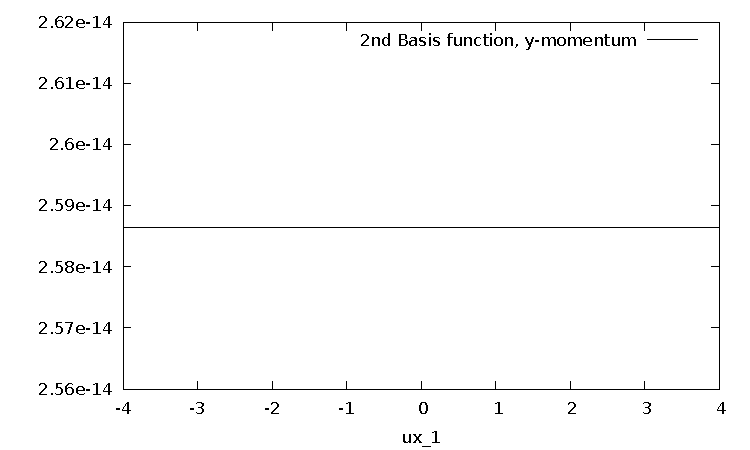
\includegraphics[scale=\zoomfactor]{{{ord1_ux1_differing_ux2_ux3/10.0_10.0_10.0_y_0.0_2.0_0.0_0.0_0.0f03}}}
  % }
  % \subfigure[] {
  %   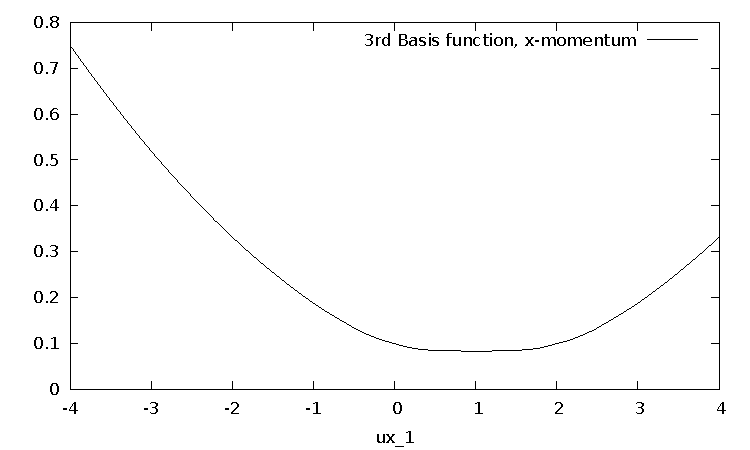
\includegraphics[scale=\zoomfactor]{{{ord1_ux1_differing_ux2_ux3/10.0_10.0_10.0_y_0.0_2.0_0.0_0.0_0.0f04}}}
  % }
  % \subfigure[] {
  %   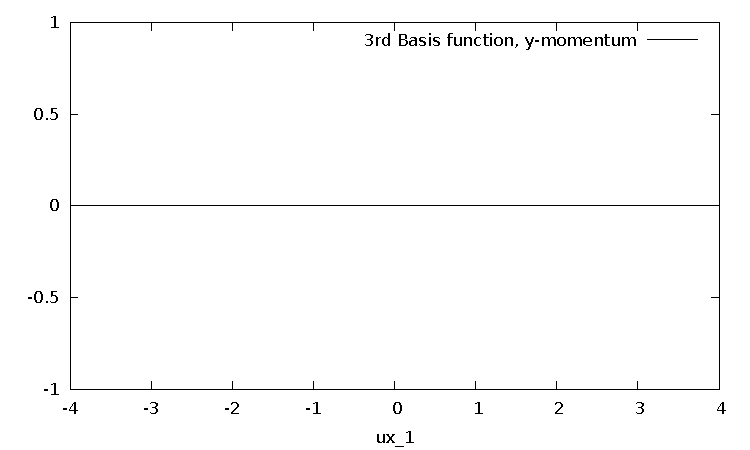
\includegraphics[scale=\zoomfactor]{{{ord1_ux1_differing_ux2_ux3/10.0_10.0_10.0_y_0.0_2.0_0.0_0.0_0.0f05}}}
  % }
\caption{}
\label{fig:ord1_ux1_differing_ux2_ux3}
\end{figure}
